\documentclass{article}
\usepackage[utf8]{inputenc}
\usepackage{url}
\usepackage{graphicx}
\usepackage{float}
\usepackage{array}
\usepackage[export]{adjustbox}
\graphicspath{ }

% code listing config
\usepackage{listings}
\lstset{
    basicstyle=\footnotesize\ttfamily,
    breaklines=true,
    tabsize=4,
    keepspaces=true,
    columns=flexible,
    % backgroundcolor=\color[gray]{0.9},
    frame=single
}

\title{Embedded Systems Laboratory 2\\
        Custom Avalon Slave Programmable Interface}
    \author{
  Snoeijs, Jan\\
    \texttt{jan.snoeijs@epfl.ch}
  \and
  Spieler, Michael\\
  \texttt{michael.spieler@epfl.ch}
}
\date{07 November 2017}

\begin{document}

\maketitle

\section{Choice of peripheral}
We have chosen to implement the slave peripheral for the W2812 LED controller. In this report we present an overview of our hardware realization of the programmable module, the full system architecture and our software code.

\section{System overview}

Figure \ref{fig:SLBD} shows the block diagram of the whole system.
It comprises a NIOS-II CPU, SRAM memory, JTAG UART and our custom LED programmable interface, which are all connected over the Avalon bus.
The LED programmable interface has, besides the Avalon slave signals, only one output signal which exits the FPGA on \verb'GPIO_0(0)'. A daisy chain of 16 WS2812 LED controllers is connected to \verb'GPIO_0(0)' which will be controlled by the custom programmable interface.

\begin{figure}[H]
    \centering
    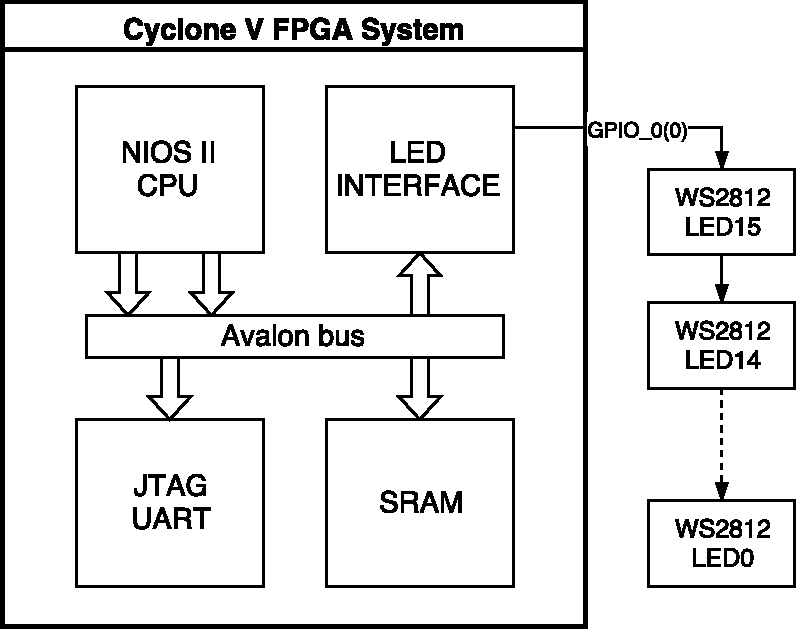
\includegraphics[width=0.7\textwidth]{system_level_block_diagram}
    \caption{System level block diagram}
    \label{fig:SLBD}
\end{figure}

Figure \ref{fig:MLBD} illustrates the Module-level block diagram of the programmable interface including the Avalon slave signals, \verb'LedData' output signal, the register set and a finite state machine which is documented in section \ref{sec:fsm}.

\begin{figure}[H]
    \centering
    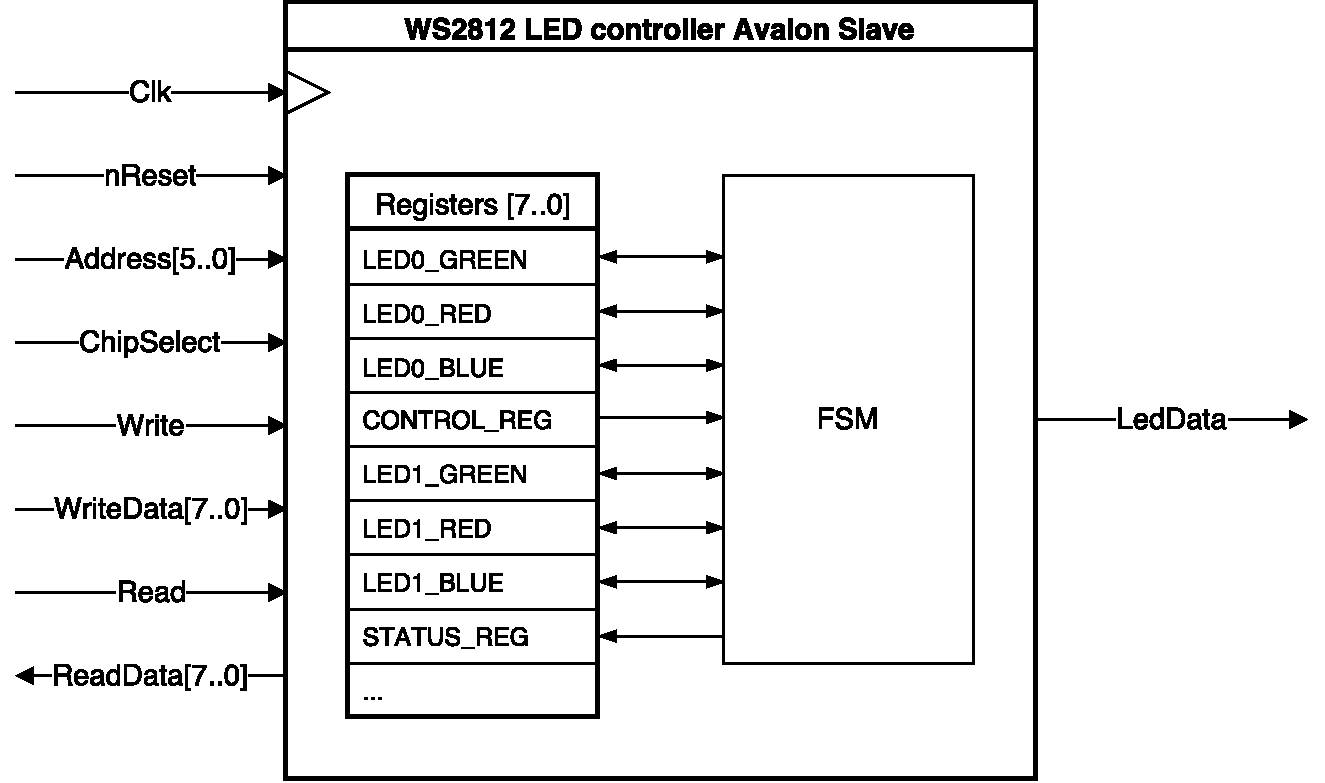
\includegraphics[width=\textwidth]{Led_periph_block_diagram}
    \caption{Module-level abstract block diagram}
    \label{fig:MLBD}
\end{figure}

\section{Finite state machine - VHDL implementation}
\label{sec:fsm}

In this section we describe the VHDL implementation of the programmable interface for the LED controller. 
The implementation we chose is the finite state machine shown in Figure \ref{fig:FSM}. 
In the IDLE state, the machine is waiting and the registers are ready to be written. 
A signal sent by the processor (software) handles the transition to the LOAD state where the data registers are written.
In this state, the Avalon bus is allowed to write in the registers.
The transition is again allowed by the software by setting the control register to 2.
From then on every write operation in the registers is not taken into account until the system is back in IDLE state.
In the WR0 and WR1 states are similar.
In WR0, a signal '0' is sent over the LedData signal ( '1' for 0.4 $\mu$s and '0' for 0.85 $\mu$s) by decrementing a counting register ("wr0 cnt"). In parallel of this, a series of counters are decremented to determine how many bits are left to write and what is the value of the next bit. This process determines whether the state machine stays in the same state, switch to the other writing state or return to IDLE.

\begin{figure}[H]
    \centering
    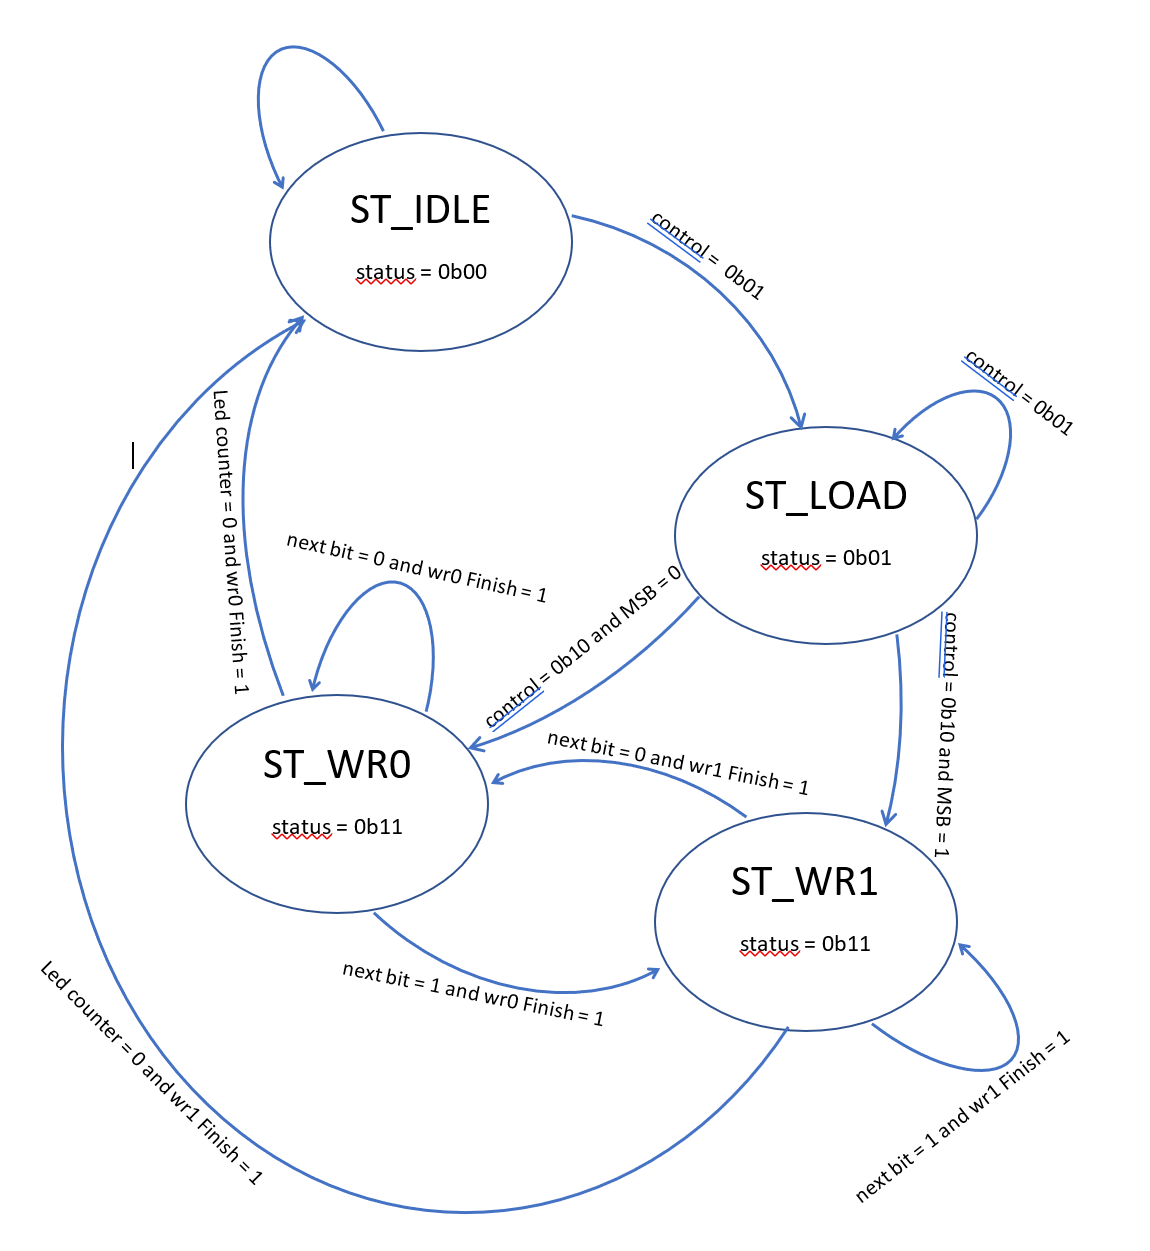
\includegraphics[width=\textwidth]{FSM}
    \caption{State diagram of slave avalon Led controller FSM}
    \label{fig:FSM}
\end{figure}


\subsection{Detailed description of the VHDL code}
Our implementation of the FSM described before in VHDL is divided into several processes. To make sure the design is synchronous we wrote two processes dependent only on clock and reset. One instantiates the state register for the FSM, and the other one instantiates all the other used registers, divided into the software-accessible registers and inaccessible internal registers.

A separate process handles the transition between the states of the FSM.

Then, outside of any process, status signals are asserted in a concurrent way. These signals are of Boolean type and toggle to ‘1’ if their associated counter has reached its final value. The processes sensitivity list are dependent on these status signals and on the registers, which shouldn't compromise the synchronization of the design because the status signals only depend on registers which behave synchronously.

In an other process we define the signal assertions that need to be done in each state of our FSM. In this process, our different counters (leds, color, bits, wr0) are decremented in a cascade way, meaning that the bit counter is decremented by one only when wr0 is fully decremented and so on.
This should ensure that the data is sent in the right order to the LEDs.

Two similar processes (WR0, WR1) define how long a pulse should last to write a '0' or a '1' in the leds. We have done this in accordance with the data sheet specifications taking tolerances into account (Table \ref{tab:1}). The reset code of 50 $\mu$s between two sets of data is handled in software.

Finally, we wrote a process for the Avalon interfacing, where the 8-bit vector stored in "WriteData" is written into our data register (array of 16x3x8 bits) depending on the "Address" and the data stored in our status register is assigned to "ReadData". All these operations happen in accordance with the Avalon bus requirements; ChipSelect and Write have to be '1' for a write and ChipSelect and Read have to be '1' for a read.

\begin{table}[H]
    \centering
    \begin{tabular}{|c||c|c|c|}
    \hline
     & nominal value [$\mu$s] & tolerance [ns] & measured value [$\mu$s] \\
    \hline
    \hline
    H1 & 0.7 & +/- 150 & 0.8 \\
    \hline
    L1 & 0.6 & +/- 150 & 0.46 \\
    \hline
    Total WR1 & 1.4 & +/-600 & 1.26 \\
    \hline
    H0 & 0.35 & +/- 150 & 0.45 \\
    \hline
    L0 & 0.8 & +/- 150 & 0.85 \\
    \hline
    Total WR0 & 1.15 & +/- 600 & 1.3 \\
    \hline
    \end{tabular}
    \caption{LED controller protocol --- specifications vs measurements}
    \label{tab:1}
\end{table}


\begin{figure}[H]
    \centering
    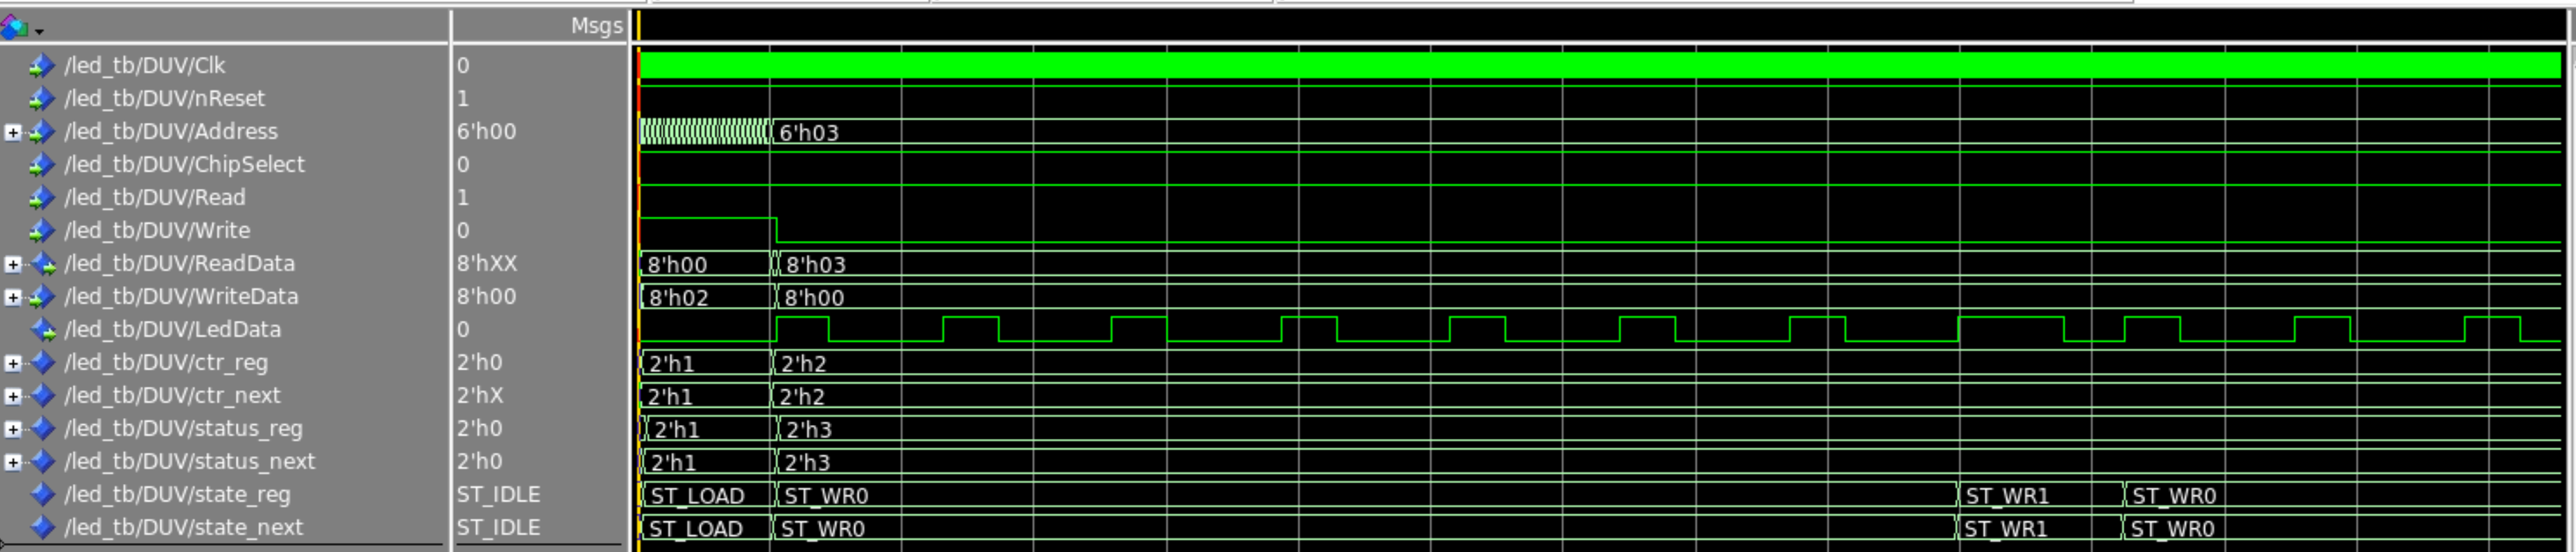
\includegraphics[width=\textwidth]{modelsim_states}
    \caption{State register behavior --- Modelsim}
    \label{fig:SRBM}
\end{figure}

\begin{figure}[H]
    \centering
    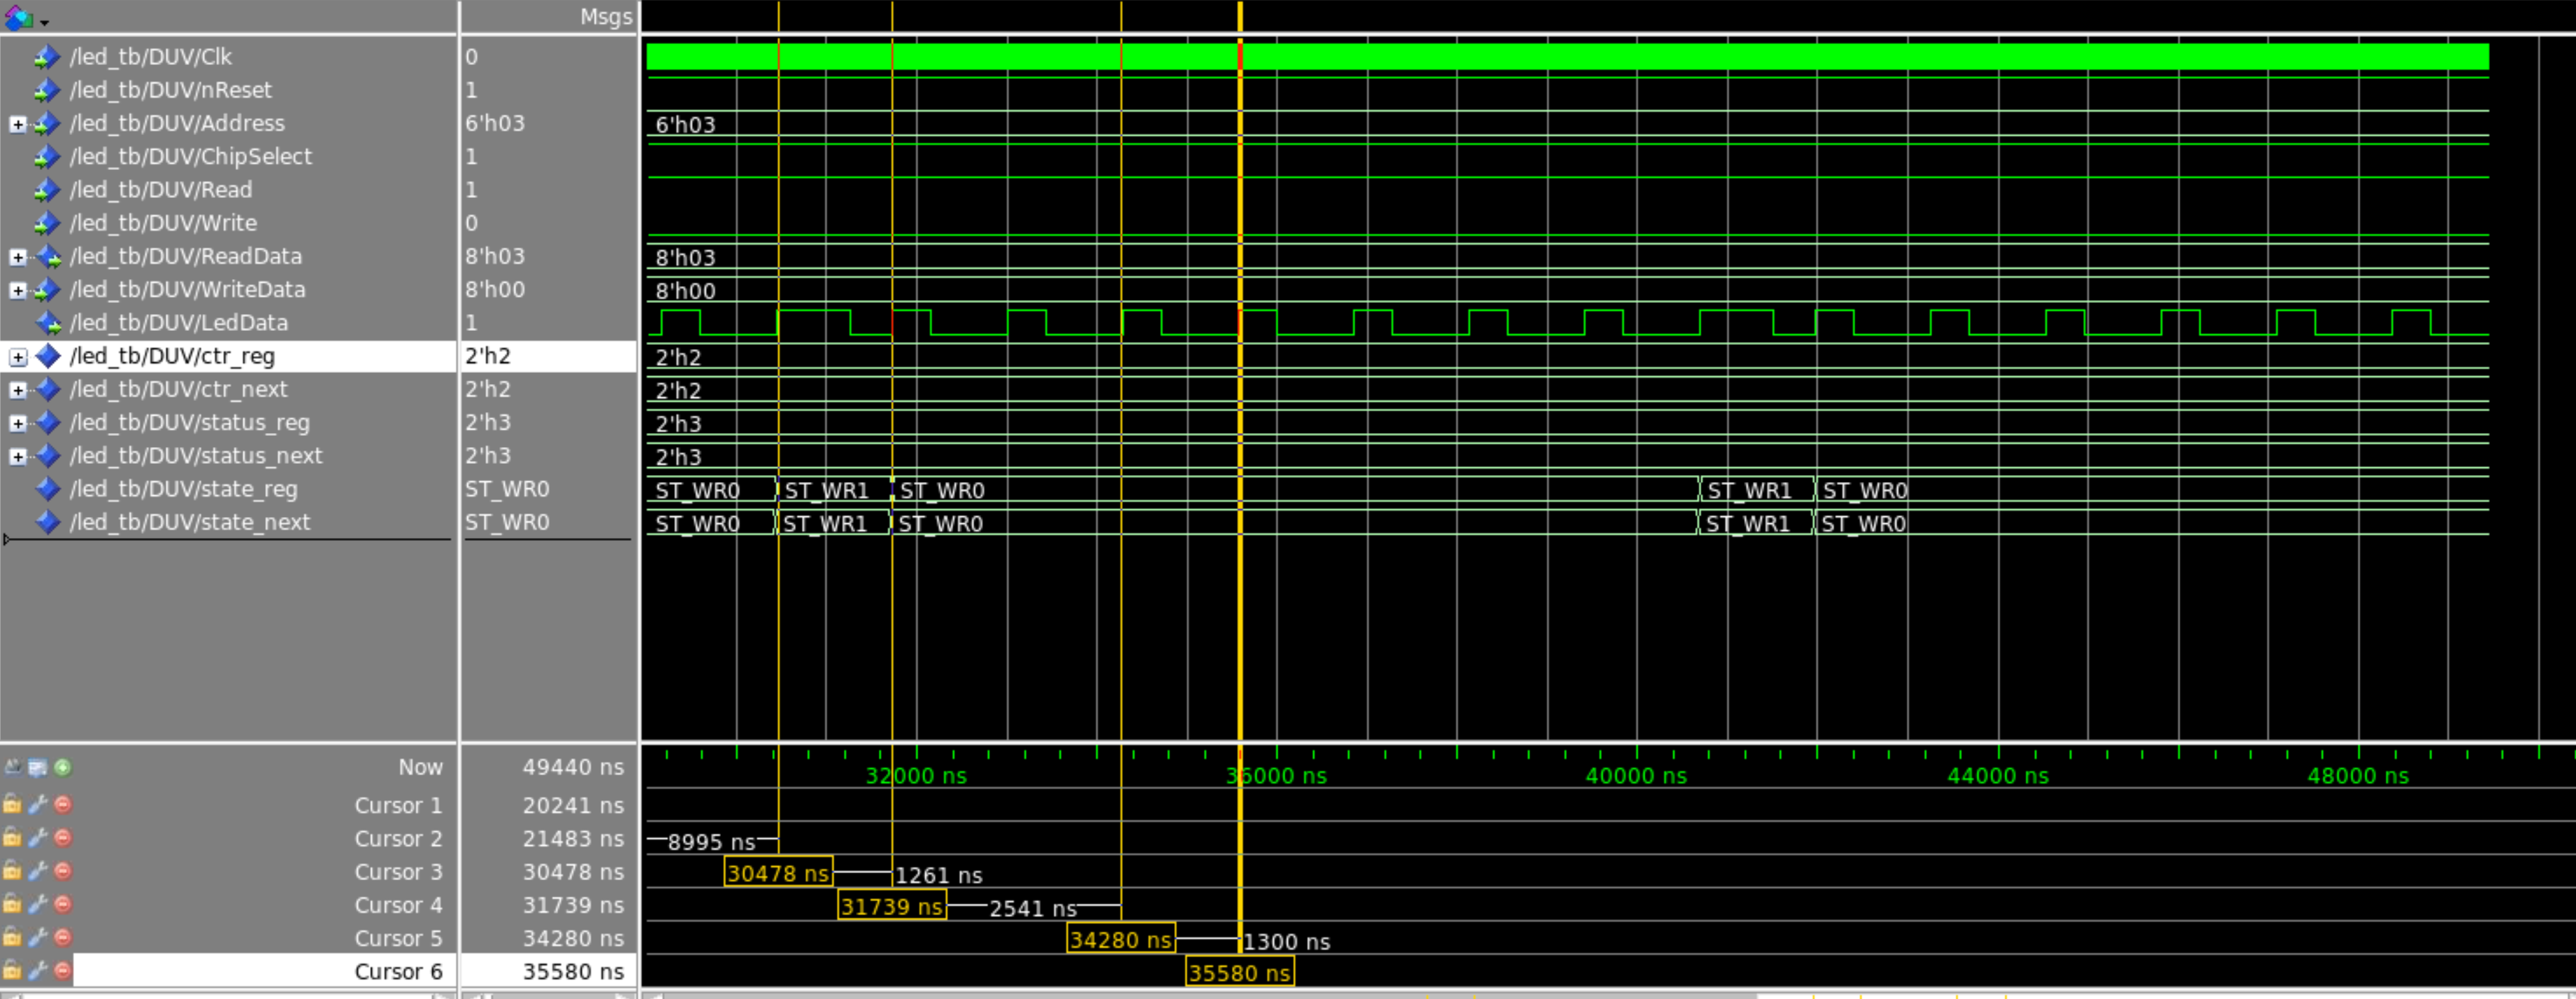
\includegraphics[width=\textwidth]{modelsim_leddata}
    \caption{Output signal behavior --- Modelsim}
    \label{fig:OSBM}
\end{figure}

Figure \ref{fig:SRBM} shows the behavior of the state register and Figure \ref{fig:OSBM} shows the output signal of the module and shows the timings of a write '1' to the LED and a write '0'.

\section{Software}

In this section we briefly describe how the programmable interface is accessed from software running on the NIOS-II processor.

\subsection{Register map}

Table \ref{tab:regs} shows the register map of the programmable interface.
\begin{table}[H]
    \centering
    
    \begin{tabular}{|c|c|c|p{70mm}|}
    \hline
     offset & register & R/W & description \\
    \hline
    \hline
     0b000000 & \verb'LED0_G' & W & 8 bit register storing the color intensity \\
     0b000001 & \verb'LED0_R' & W & -- \\
     0b000010 & \verb'LED0_B' & W & -- \\
     0b000011 & \verb'CR' & W & 2 bit control register with 2 defined values: \verb'0b01' start writing, \verb'0b10' finished writing \\
     0b000100 & \verb'LED1_G' & W & -- \\
     0b000101 & \verb'LED1_R' & W & -- \\
     0b000110 & \verb'LED1_B' & W & -- \\
     0b000111 & \verb'SR' & R & 2 bit status register with 3 defined values: \verb'0b00' ready, \verb'0b01' waiting for data, \verb'0b11' busy \\
     0b001000 & \verb'LED2_G' & W & -- \\
     0b001001 & \verb'LED2_R' & W & -- \\
     0b001010 & \verb'LED2_B' & W & -- \\
     0b001011 & Unused & W & -- \\
     ... & ... & ... &  -- \\
     ... & ... & ... & -- \\
     0b111100 & \verb'LED15_G' & W & -- \\
     0b111101 & \verb'LED15_R' & W & -- \\
     0b111110 & \verb'LED15_B' & W & -- \\
     0b111111 & Unused & W & -- \\
     \hline
     
\end {tabular}
\caption{Register map of the LED interface}
\label{tab:regs}
\end{table}

\paragraph{LED data register} The LED data registers are 4 byte aligned where \verb'LEDx' has the offset \verb'0bxxxx00'.
Each LED has 3 8bit data registers: \verb'LEDx_G' with offset \verb'0b00', \verb'LEDx_R' with offset \verb'0b01' and \verb'LEDx_B' with offset \verb'0b10'. The offsets \verb'0bxxxx11' are unused except for the control register \verb'CR' which is at offset \verb'0b000011' and the status register which is at offset  \verb'0b000111'.

\paragraph{Control Register}
The control register is 2 bit wide. Before writing LED data, the value \verb'0b01' must be written to \verb'CR'. Then the value \verb'0b01' must be written to initiate the transmission.

\paragraph{Status Register}
The status register is 2 bit wide and represents the state of the programmable interface:
\verb'0b00' ready, \verb'0b01' waiting for data, \verb'0b11' busy.
The software can poll the status register to detect when the transmission is complete.


\subsection{Source Code}

The source listing \ref{lst:main_c} shows a simple demo program that turns on a green LED wich propagates along the LED strip. The register map is represented through C macros defined at line 12. On line 42 the load command is written to the control register followed by the LED data write. The data write is finished by writing the start command to the control register on line 56. Then on line 59 the program polls the status register until the transmission was successful. On line 61 we inserted a delay long enough to let the transmitted data be updated to the corresponding LED and to obtain a visible animation.

\begin{lstlisting}[
    language=C++,
    numbers=left,
    caption=main.c,
    label=lst:main_c
]
/*
Title: Lab2 LED Programmable interface
Authors: Jan Snoeijs, Michael Spieler
*/

#include <inttypes.h>
#include <stdio.h>
#include <system.h>
#include <io.h>

// LED register access defines
#define LED_RED(N)      (4*(N) + 1)
#define LED_GREEN(N)    (4*(N) + 0)
#define LED_BLUE(N)     (4*(N) + 2)
#define BLINKY_CR       3
#define BLINKY_SR       7

// LED CR & SR bitmask
#define BLINKY_CR_LOAD  0x01
#define BLINKY_CR_START 0x02
#define BLINKY_SR_BUSY  0x03

void delay(uint64_t n)
{
    while (n-- > 0) {
        asm volatile ("nop");
    }
}

void led_write_data(unsigned i, uint8_t R, uint8_t G, uint8_t B)
{
    IOWR_8DIRECT(BLINKY_0_BASE, LED_RED(i), R);
    IOWR_8DIRECT(BLINKY_0_BASE, LED_GREEN(i), G);
    IOWR_8DIRECT(BLINKY_0_BASE, LED_BLUE(i), B);
}

int main()
{
    unsigned active_led = 0;;
    while (1) {
        // enter state LOAD
        IOWR_8DIRECT(BLINKY_0_BASE, BLINKY_CR, BLINKY_CR_LOAD);

        // fill data
        unsigned int i;
        for (i = 0; i < 16; i++) {
            if (i == active_led) {
                led_write_data(i, 0, 0xff, 0);
            } else {
                led_write_data(i, 0, 0, 0);
            }
        }
        active_led = (active_led + 1) % 16;

        // start sending
        IOWR_8DIRECT(BLINKY_0_BASE, BLINKY_CR, BLINKY_CR_START);

        // wait until done
        while(IORD_8DIRECT(BLINKY_0_BASE, BLINKY_SR) == BLINKY_SR_BUSY);

        delay(100000);
    }
}
\end{lstlisting}

\end{document}
